\chapter{Introduction} \label{chap:intro}

\iffalse
\section{Preparing your dissertation} \label{sect:thefirst}

You are strongly encouraged to use the Latex templates provided.

\subsection{Paper}
The manuscript should be in A4 size, and the printed paper should
be of at least 70 gsm.

\subsection{Font and margins}
Thesis should be printed on both sides of the paper. Use no less
than 1.5 spacing, with quotations and notes single-spaced.
Regarding \textbf{Character size}, not less than 2.0mm for
capitals and 1.5mm for x-height (the height of a lower-case x). Us
a serif font (i.e. Times) between 10 and 12 points. Use consistent
and clear fonts through all the document.

The text layout should be approximately as follows:

\begin{itemize}
    \item $4cm$ binding margin
    \item $2cm$ head margin (top of page)
    \item $2.5cm$ fore-edge margin
    \item $4cm$ tail margin (bottom of page)
\end{itemize}

\fi




% \section{Title Page}

% \iffalse
% The title page should contain the title of thesis, authors name,
% and at the foot of the page: the name of degree,  Your University,
% and the year of presentation. Something like this:
% \fi

% \vspace*{1cm}
% \begin{center}
% {\Large\bf Optimized Waypoints selection for UAV maximum area coverage\\} \vspace{2cm} {\large
% Mark Bastourous\\
% \vspace{1cm}
% Laboratoire d'Electronique,Informatique et Image \\
% Universite De Bourgogne}

% \end{center}



% \vspace{2cm}
% \begin{center}
% {\large A Thesis Submitted for the Degree of MSc Computer vision and Robotics Univesite De Bourgogne\\ \vspace{0.3cm} $\cdot$ 2016 $\cdot$}
% \end{center}

% \iffalse
% \subsection{References}
% You can reference other authors by using the $cite command$
% \cite{Pokorski:1998hr}. You are encouraged to use bib files and
% let bibtex do the job for you.
% \fi

\section{INTRODUCTION}

Aerial robots have grown great attention in the last decades due to its capabilities in solving many problems in many domains. They are still under study, investigation and development because of the several constrains and challenges that are in software and hardware of its construction on  many levels and layers. 

Some of the software challenges are state estimation, control, decision making, mapping, and path planning. Some of the hardware challenges are the weight/load ratio, power source, sensors, etc. 

There are various applications that practically make use of unmanned aerial vehicles (UAV) and much more are still under study and development in the research labs and institutes. These applications are covering many fields of interest in both civilian and military purposes. Some of these practical applications are search and rescue, inspections, surveillance, photography, agricultural terrain mapping, mineral exploration, etc. Some prospective applications like medical cargo delivery because it will not rely on the normal road maps if they exist, or traffic constrains.

There are many types of UAVs categorized based on the geometry and designs like fixed wing, flapping wing, and rotor crafts, mentioned in more details in \cite{UAV_general}. Figure \ref{fig:micro_aerial}  shows some of the current UAVs. From cheap and small toys that you can be bought anywhere as the RC planes, toy quadcopter, to big military projects such as the Global Hawk.

\begin{figure}[!htb]
\minipage{0.80\textwidth}
  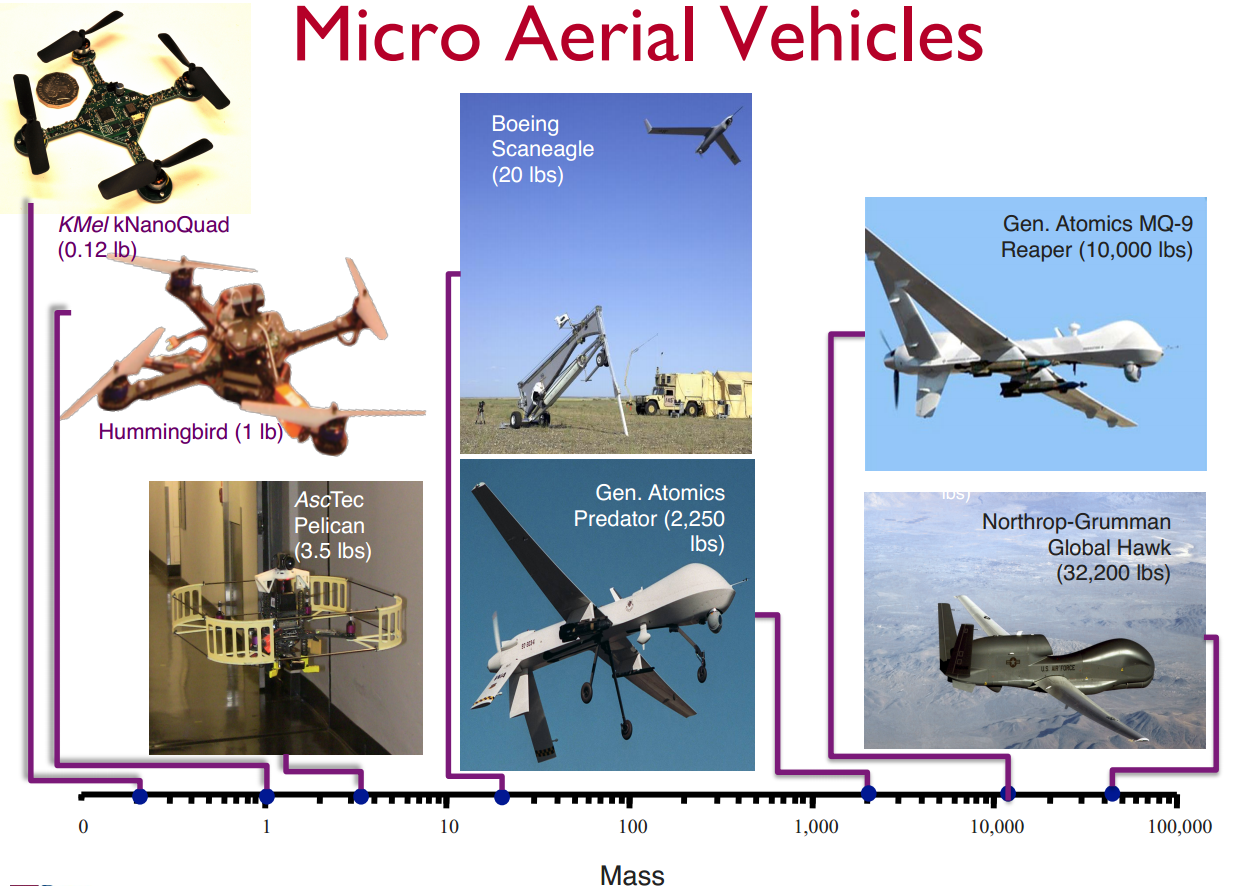
\includegraphics[width=\linewidth]{figures/Micro_aerial.png}
  \caption{Micro aerial vehicle}\label{fig:micro_aerial} 
  \endminipage\hfill
\end{figure}

 

UAVs have recently reached a decline in their cost especially the quadcopters. In this thesis during the practical implementation part, quadcopters as one type of the rotor crafts will be used. The quadcopter used is Ar.drone 2.0 from the french company Parrot. It is off shelf drone that can be found on the market with comparable cheap price in range of 300 euros depending on the extras. It has been used several times in research labs and studied like in \cite{Ardrone1},\cite{Ardrone2},etc.

There are many advantages that make quadcopter as a specific type of UAVs, suitable for both indoor and outdoor applications. It takes off vertically, do not need a runway, hover in its place, comparably light weight, and small in size.

For simulation V-REP with a model of quadcopter available was used. Some modification in this model was introduced to cope with the problem being solved and will be discussed later in more details. In both the practical work and simulation, ROS packages were used, tuned and implemented to control the quadcopter.

% There was no embedded systems work done and offshelf usage of the drone was utilized.

Some of the previously mentioned applications require area coverage of outdoor or indoor mapping. Coverage path planning is an active research topic as the sub division of the general path planning problem that is studied by robotics domain for several decades till our day. It has been applied on many platforms in many areas where these platforms work. Normally the area to be covered is not a regular one. Most of the literature review that comes to the awareness to the author of this thesis are concerned with uniform areas and prior map with static or dynamic obstacles. Platforms here means the mobile robots like autonomous underwater vehicles(AUV), unmanned aerial vehicle(UAV), or ground vehicles. 

% Aerial robots is still under study, investigation and development because of the many constrains and challenges that are in software and hardware of its construction on  many levels and layers. 

Prior information about the environment is assumed to be given in the form of a rough map for the area required to be covered. For this work, we model the set of coverage problems as arc routing problems. Although these routing problems are generally NP-hard, our approach aims for optimal solutions through the use of low-complexity algorithms in a branch-and-bound framework when time permits and approximations when time restrictions apply.


The final objective of this thesis research is to design a global optimization scheme allowing a cameras network to be self organized or to plan single trajectory of a flying robot equipped with a camera, according to fixed priority and constraints, in order to ensure a full coverage of a given scene. Applicable solution for both indoor and outdoor with ensuring coverage of the terrain while minimizing path repetition. Then building a mosaicking of the area covered and compare it with the original scene.


% %\textcolor{davidS}
% {The main problem of UAVs is the autonomy of fly, because of the battery run-time. This short time action restrained the possibility to use a set of UAVs and the work cooperation for a long time surveillance if there is no much UAVs available at the moment}. One smarter possibility is to create a monitoring path with several UAVs which  %\textcolor{davidS}
% {alternately automatically relays when the battery is low.} 
% During the navigation of the UAV's path, it is possible to get the image of the area to survey and build the mosaic of the area. 
% This paper will focus on finding the best waypoints for the UAV to pass through, to reduce the computation usually done in the path planning and coverage process. In order to find a good path to cover most of the area the essential point is to propose the best waypoints. %Finding the waypoint can be reduced to the problem of finding the best coverage.

% ensures complete coverage of the terrain while minimizing path repetition indoor gps denied  slam methods were used to localize and navigate the UAV using the visual 

In the next subsection the objectives of this thesis will be discussed.

\subsection{Objectives}
\begin{itemize}

\item Study coverage path planning problem, implement the suitable one.
\item Examine and validate the path planning in both simulation and real world with practical hardware.
\item Construct a final mosaicked scene after the UAV acquire images.

\end{itemize}

\subsection{Thesis Organization}
This thesis is organized as follows. Chapter 2 discusses the background and shows the literature review done by the author. Then comes the description of the methodology which is written into two chapters; 3 and 4. In chapter 3, the methods of selecting the best waypoints is discussed. Chapter 4 contains the path planning methods developed and used. Also explanation of the combining several methods is provided. The whole pipeline is being presented by the end of this chapter too. Results and experiments in both real life and simulation is discussed and shown in chapter 5. Finally conclusion and future work are addressed in chapter 6. 